\documentclass{beamer}

\usepackage{Vor2018glærur}

\title{Ólínuleg Bestun}
\subtitle{Fyrirlestur 2}

\begin{document}

\begin{frame}
\titlepage
\end{frame}

\section{Hólfavigrar}

\begin{frame}[fragile]{Hólf}
    ``Venjuleg'' Matlab fylki eiga erfitt með að geyma óregluleg gögn, t.d. mislanga strengi.

    Búa má til hólfafylki (e. \emph{cell array}) með því að umlykja gögnin sem geyma skal með slaufusvigum:
    
\begin{minted}[frame=lines]{matlab}
>> cells = {'a', 'ab', 'abc', 1}
cells = 
    'a'    'ab'    'abc'    [1]
>> whos cells
    Name       Size    Bytes  Class    Attributes
    cells      1x4       468  cell
\end{minted}
\end{frame}

\begin{frame}[fragile]{Hólfafylki - dæmi}
    Fyrri skipunin býr til $1\times 4$ hólfavigur, sú seinni $2 \times 2$ hólfafylki
\begin{minted}[frame=lines]{matlab}
>> ca = {23, 'a', 1:2:9, 'hello'} 
ca = 
    [23]   'a'   [1x5 double]   'hello'

>> cm = {23, 'a'; 1:2:9, 'hello'}
cm = 
    [        23]    'a'    
    [1x5 double]    'hello'
\end{minted}
\end{frame}

\begin{frame}[fragile]{Vísun í hólfavigra}
    \begin{center}
    Getum vísað í stök hólfavigra á tvo vegu
    \end{center}
    
    \begin{columns}
    \column{0.5\textwidth}
    Með innihaldsvísun (e. \emph{content indexing}), sem gefur okkur innihald hólfsins
\begin{minted}[frame=lines]{matlab}
>> ca{3}
ans =
    1    3    5    7    9
\end{minted}
    \column{0.5\textwidth}
    Með hólfavísun (e. \emph{cell indexing}), sem gefur okkur hólfið sem er á þeim stað
\begin{minted}[frame=lines]{matlab}
>> ca(3)
ans = 
    [1x5 double]
\end{minted}
    \end{columns}
\end{frame}

\section{Fallshandföng og nafnlaus föll}

\begin{frame}[fragile]{Nafnlaus föll}
    \begin{itemize}
        \item Nafnlaus föll (e. \emph{anonymous functions}) eru einföld einnar línu föll, sbr. lambdas í öðrum forritunarmálum
         \begin{itemize}
            \item Skilgreind eins og breytur, ekki í sérstakri \texttt{.m}-skrá
         \end{itemize}
        \item Almennt snið:
\begin{verbatim}
handfang = @(viðföng) fallsegð
\end{verbatim}
        \begin{itemize}
            \item Þar sem \texttt{handfang} er fallshandfang (e. \emph{function handle})
            \item \texttt{viðföng} er 0 eða fleiri breytur sem unnið er með
            \item \texttt{fallsegð} er ein Matlab-segð
        \end{itemize}
    \end{itemize}
\end{frame}

\begin{frame}[fragile]{Fallshandföng}
\begin{itemize}
    \item Fallshandfang er leið til að vísa til falls
    \begin{itemize}
        \item Koma líka fyrir í öðrum samhengjum en þegar nafnlaus föll eru búin til
    \end{itemize}
    \item Getum fengið handfang fyrir ýmis föll (þar á meðal innbyggð)
    \begin{itemize}
        \item Notum til þess virkjann (e. \emph{operator}) @
    \end{itemize}
\end{itemize}
\begin{minted}{matlab}
    >> sinHandle = @sin
    sinHandle = 
        @sin
    >> sinHandle(pi/4)
    ans =
        0.7071
\end{minted}
\end{frame}

\section{Einföld teikniföll}

\begin{frame}[fragile]{\texttt{fplot} fallið}
    Fallið \texttt{fplot} teiknar fall á gefnu bili. Almennt snið:
    \begin{verbatim}
    >> fplot(fallshandfang, [minnstaX stærstaX])
    \end{verbatim}
    Fallið sem handfangið vísar til verður að taka við einu gildi og skila einu gildi. Það verður líka að ráða við að inntakið sé vigur.
\end{frame}

\begin{frame}[fragile]{Teiknifallið plot}
    \begin{columns}
    \column{0.5\textwidth}
        \begin{itemize}
            \item Mest notaða teiknifallið er \texttt{plot}
            \begin{itemize}
                \item Tekur inn vigra fyrir $x$ og $y$ og teiknar línurit
                \item Ásarnir eru kvarðaðir sjálfkrafa
            \end{itemize}
        \end{itemize}
\begin{minted}[frame=lines]{matlab}
>> x = 1:6;
>> y = randi([0, 10],1,6);
>> plot(x,y)
\end{minted}
\column{0.5\textwidth}
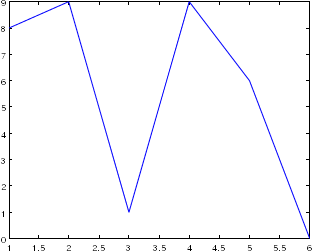
\includegraphics[width=\linewidth]{../T1a/Pics/plot-example5}
\end{columns}
\end{frame}

\begin{frame}{Ýmsar stillingar á plot}
    \begin{columns}
        \column{0.6\textwidth}
        \begin{itemize}
            \item Hægt er að setja kvarða á ásana:
            \begin{itemize}
                \item \texttt{>> axis([1, 6, 0, 12])}
                \item Sniðið er \texttt{[xmin, xmax, ymin, ymax]}
            \end{itemize}
            \item Setja má merki á ásana:
            \begin{itemize}
                \item \texttt{>> xlabel('Nemandi')}
                \item \texttt{>> ylabel('Einkunn')}
            \end{itemize}
            \item Titill á línuritið:
            \begin{itemize}
                \item \texttt{>> title('Nemendur og einkunnir')}
            \end{itemize}
            \item Hægt er að skrifa ``ofan í'' sömu myndina með því að gefa skipunina \texttt{hold on} 
        \end{itemize}
        
        \column{0.4\textwidth}
        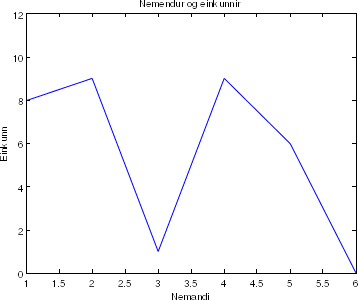
\includegraphics[width=\linewidth]{../T1a/Pics/plot-example6}
    \end{columns}
\end{frame}
    
\begin{frame}{Stillingar línurits}
    \vspace{\baselineskip}
    3. viðfangið í plot fallinu eru stafir sem lýsir gerð línuritsins.\footnote{Sjálfgefin stilling er \texttt{plot(x, y, 'b -')}}\\
    \texttt{>> plot(x, y, '}\emph{lmt}\texttt{')} $\leftarrow$ \textbf{l}itur, \textbf{m}erki, \textbf{t}egund.\\
    \vspace{0.5\baselineskip}
    \begin{columns}
    \small
    \column{0.33\textwidth}
    \begin{tabular}{cl}
    \toprule
    Merki&Litur\\
    \midrule
    \texttt{b}&blár\\
    \texttt{g}&grænn\\
    \texttt{r}&rauður\\
    \texttt{c}&blágrænn\\
    \texttt{m}&blárauður\\
    \texttt{y}&gulur\\
    \texttt{k}&svartur\\
    \bottomrule
    \end{tabular}
    \column{0.33\textwidth}
    \begin{tabular}{cl}
    \toprule
    Merki&Útkoma\\
    \midrule
    \texttt{.}&punktur\\
    \texttt{o}&hringur\\
    \texttt{x}&x-tákn\\
    \texttt{+}&plús-tákn\\
    \texttt{*}&stjarna\\
    \texttt{s}&ferningur\\
    \texttt{d}&tígull\\
    \texttt{v}&þríhyrningur\\
    \texttt{\^{}}&þríhyrningur\\
    \bottomrule
    \end{tabular}
    \column{0.33\textwidth}
    \begin{tabular}{cl}
    \toprule
    Merki&Tegund\\
    \midrule
    \texttt{-}&heil lína\\
    \texttt{:}&punktalína\\
    \texttt{-.}&strik-punktur\\
    \texttt{--}&strikalína\\
    \texttt{ }&engin lína\\
    \bottomrule
    \end{tabular}
    \end{columns}
\end{frame}

\begin{frame}[fragile]{Samsettar myndir}
    \begin{columns}
        \column{0.4\textwidth}
        \inputminted[frame=lines, label=subplotexample.m, fontsize=\scriptsize]{matlab}{../T1a/Code/subplotexample.m}
        \column{0.6\textwidth}
        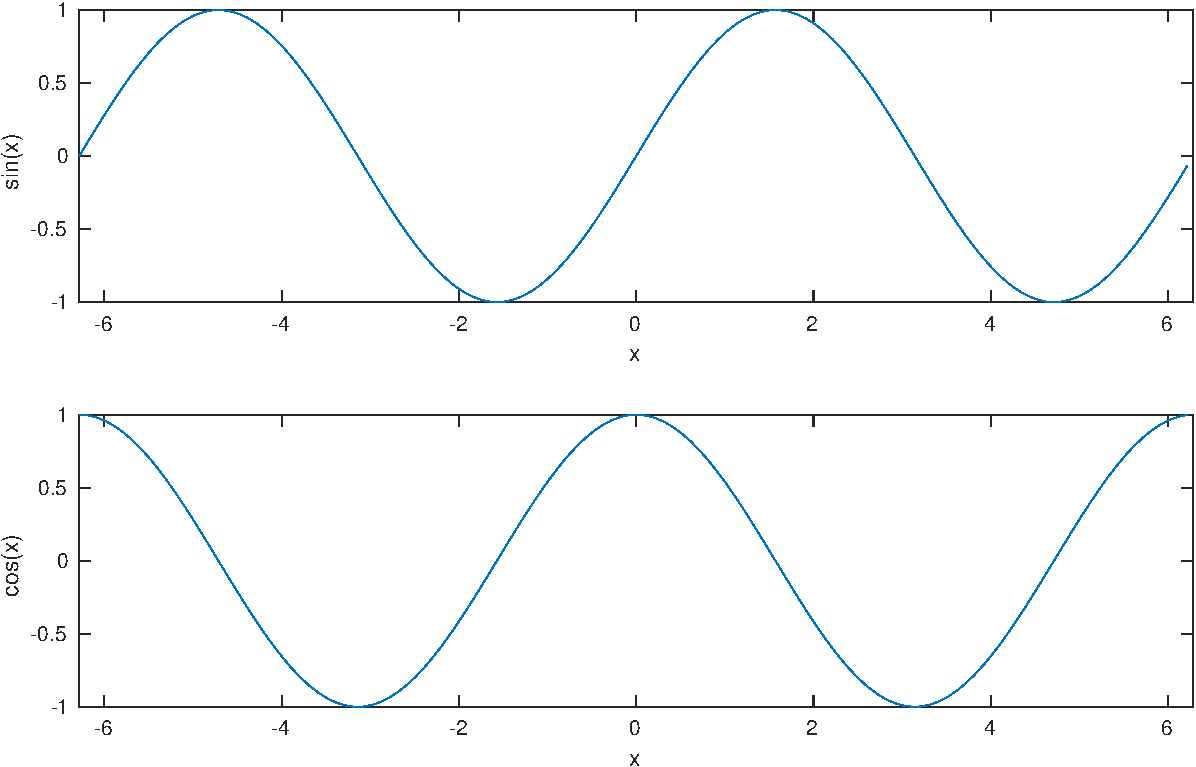
\includegraphics[width=\textwidth]{../T1a/Pics/subplot-example.pdf}
    \end{columns}
\end{frame}

\begin{frame}{Ættingjar plot-fallsins}
    \begin{itemize}
        \item Nokkur föll eru til sem hafa mjög svipaða virkni og \texttt{plot}
        \begin{itemize}
            \item \texttt{bar} gerir súlurit
            \item \texttt{area} fyllir undir ferli
            \item \texttt{stem} gerir stofnteikningu
            \item \texttt{errorbar} bætir við óvissubilum
        \end{itemize}
        \item Fleiri gerðir teiknifalla:
        \begin{itemize}
            \item \texttt{pie}
            \item \texttt{histogram}
            \item \texttt{scatter}
        \end{itemize}
    \end{itemize}
\end{frame}

\section{Þrívíddarteikning}

\begin{frame}{Yfirborðsteikningar}
    \begin{itemize}
        \item Föllin \texttt{mesh} og \texttt{surf} búa til þrívíddarmyndir af yfirborðum
        \item Taka við þremur viðföngum
        \begin{itemize}
            \item Fylki af \texttt{x}-hnitum
            \item Fylki af \texttt{y}-hnitum
            \item Fylki af \texttt{z}-hnitum (hæð yfir $xy$-sléttunni)
        \end{itemize}
        \item Fallið \texttt{contour} er hliðstætt, en teiknar hæðarlínur
    \end{itemize}
\end{frame}
    
\begin{frame}[fragile]{Dæmi um \texttt{mesh}}
    \vspace{1cm}
    Teiknum upp fallið $xe^{-x^2-y^2}$

\begin{minted}{matlab}
>> [x y] = meshgrid(-2:0.2:2, -1.5:0.2:1.5);
>> z = x.*exp(-x.^2 - y.^2);
>> mesh(x,y,z)
\end{minted}
    
    \begin{center}
    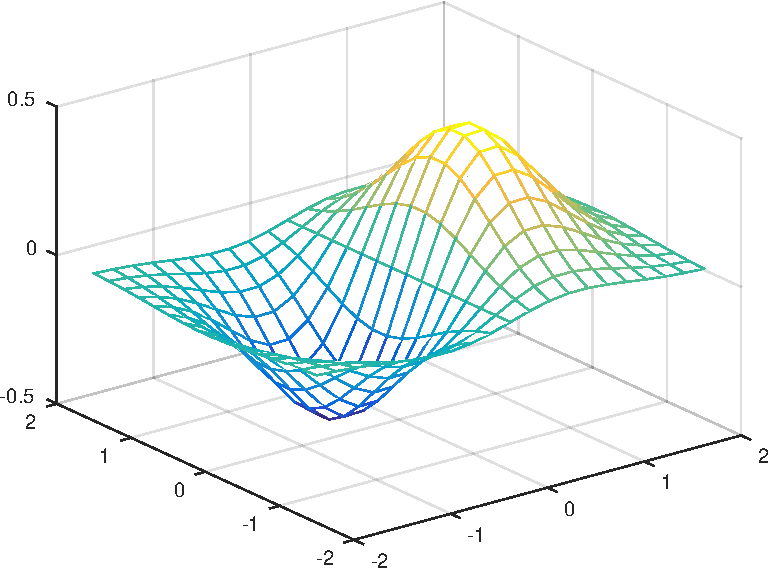
\includegraphics[width=0.4\linewidth]{../T1a/Pics/3dmesh}
    \end{center}
\end{frame}

\section{Nálgun}

\begin{frame}[fragile]{Nálgun gagnapunkta}
    Getum notað Matlab-fallið \texttt{polyfit} til að nálga gagnapunkta
    \begin{minted}[frame=lines, fontsize=\small]{matlab}
>> wind = [15.2 17.2 15.4 17.5 13.4 9.8 1.6 3.5];
>> time = 3:3:24;
>> plot(time, wind, 'r*');
>> axis([0 26 0 20])
>> lineEquation = polyfit(time, wind, 1)
lineEquation =
    -0.7175   21.3857
>> line = polyval(lineEquation, time);
>> hold on
>> plot(time, line)
    \end{minted}
    Hér reyndist besta línan vera $y = -0.7175x + 21.3857$
\end{frame}

\begin{frame}[fragile]{Besti fleygbogi}
    \begin{minted}[frame=lines, fontsize=\small]{matlab}
>> parabolicEquation = polyfit(time, wind, 2);
>> xi = linspace(min(time),max(time));
>> parabola = polyval(parabolicEquation, x);
>> plot(time, wind, 'r*', xi, parabola, 'b-')
>> axis([0 26 0 20])
    \end{minted}
    \begin{columns}
    \column{0.5\textwidth}
    \small
    Athugum: Þurfum hærri upplausn á fleygboganum til að myndin komi vel út
    
    Trix: Plot getur teiknað marga ferla í einu
    \column{0.5\textwidth}
    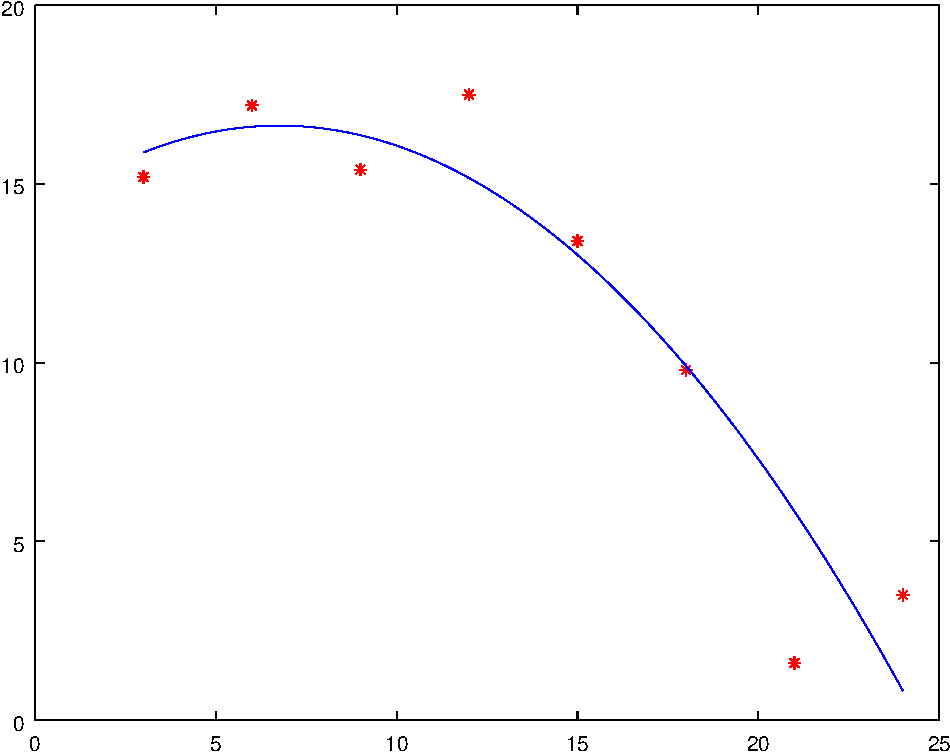
\includegraphics[width=\linewidth]{../T1a/Pics/wind-parabola}
    \end{columns}
\end{frame}

\begin{frame}{Fyrirlestraræfing 2}
    \begin{columns}
        \column{0.6\textwidth}
        \begin{enumerate}
            \item Notið \texttt{fplot} til að teikna $f(x) = x\cos(5x)$ á bilinu 0 til 10.
            \item Hér til hliðar eru hitamælingar fyrir septemberdag í Reykjavík. Teiknið snyrtilegt línurit fyrir hitastigið þennan dag.
            \item Teiknið fallið
            \[
            \frac{\sin(\sqrt{x^2 + y^2})}{\sqrt{x^2 + y^2}}
            \]
            á bilinu $-6\pi$ til $6\pi$ fyrir $x$ og $y$.
        \end{enumerate}
        \column{0.4\textwidth}
        \begin{center}
        \begin{tabular}{ll}
        \toprule
        Klst&$C^\circ$\\
        \midrule
        0&12.5\\
        3&12.4\\
        6&12.3\\
        9&12.8\\
        12&13.4\\
        15&14\\
        18&13.1\\
        21&12.8\\
        \bottomrule
        \end{tabular}
        \end{center}
    \end{columns}
\end{frame}

\end{document}
